% Esquema del ECP-730 en configuración atractiva (notación de la tesis).
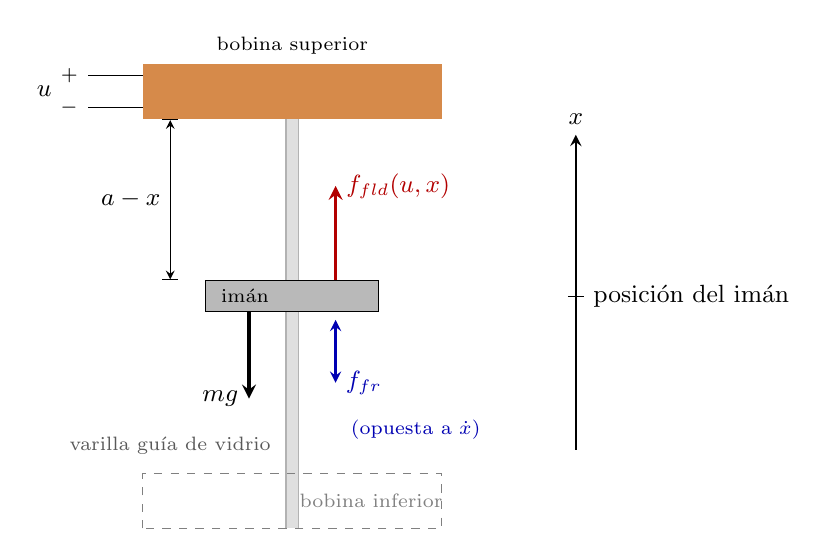
\begin{tikzpicture}[>=stealth, font=\small]
  \definecolor{cobre}{RGB}{214,138,74}
  % varilla guía
  \fill[gray!25] (-0.08,-3.6) rectangle (0.08,2.15);
  \draw[gray!60] (-0.08,-3.6) -- (-0.08,2.15) (0.08,-3.6) -- (0.08,2.15);
  \node[gray!70!black, anchor=east, font=\scriptsize] at (-0.15,-2.55) {varilla guía de vidrio};
  % bobina superior (activa)
  \fill[cobre] (-1.9,1.6) rectangle (1.9,2.3);
  \node[above, font=\scriptsize] at (0,2.3) {bobina superior};
  \draw (-1.9,2.15) -- (-2.6,2.15) node[left, font=\scriptsize] {$+$};
  \draw (-1.9,1.75) -- (-2.6,1.75) node[left, font=\scriptsize] {$-$};
  \node at (-3.15,1.95) {$u$};
  % bobina inferior (inactiva en esta configuración)
  \draw[dashed, gray] (-1.9,-3.6) rectangle (1.9,-2.9);
  \node[gray, font=\scriptsize] at (1.0,-3.25) {bobina inferior};
  % imán levitante
  \fill[gray!55] (-1.1,-0.85) rectangle (1.1,-0.45);
  \draw (-1.1,-0.85) rectangle (1.1,-0.45);
  \node[font=\scriptsize] at (-0.6,-0.65) {imán};
  % fuerzas
  \draw[->, very thick, red!70!black] (0.55,-0.45) -- (0.55,0.75) node[right] {$f_{\text{fld}}(u,x)$};
  \draw[->, very thick] (-0.55,-0.85) -- (-0.55,-1.95) node[left] {$mg$};
  \draw[<->, thick, blue!70!black] (0.55,-0.95) -- (0.55,-1.75) node[right] {$f_{\text{fr}}$};
  \node[blue!70!black, font=\scriptsize, anchor=north west] at (0.62,-2.1) {(opuesta a $\dot x$)};
  % distancia a la bobina
  \draw[|<->|, thin] (-1.55,-0.45) -- (-1.55,1.6) node[midway, left] {$a-x$};
  % eje x
  \draw[->, thick] (3.6,-2.6) -- (3.6,1.4) node[above] {$x$};
  \draw (3.5,-0.65) -- (3.7,-0.65) node[right] {posición del imán};
\end{tikzpicture}
